\section{Empirical Evaluation \& Benchmarking}
\label{sec:evaluation}

This section presents a comprehensive quantitative evaluation of FedGuard. We evaluate the performance overhead, security efficiency, Byzantine attack mitigation, dynamic regulatory compliance, and deep learning workload scalability of the governance control plane across multi-organizational federated environments.

\subsection{Experimental Setup and Benchmark Methodology}

\subsubsection{System Environment and Workload Configuration}
Experiments were conducted on a high-performance distributed benchmark environment simulating up to 20 institutional nodes. Each node operates as an isolated participant communicating with the governance control plane over TLS 1.3 encrypted channels.

To evaluate real-world performance, we deploy a production-grade PyTorch deep learning workload:
\begin{itemize}
    \item \textbf{Model Architecture:} ResNet-18 image classification neural network containing 11.17 million trainable parameters ($d \approx 11.17 \times 10^6$).
    \item \textbf{Dataset \& Partitioning:} CIFAR-10 dataset partitioned deterministically across nodes using a Dirichlet distribution $\text{Dir}(\alpha=0.5)$ to reflect realistic non-IID statistical heterogeneity.
\end{itemize}

\subsubsection{Evaluation Baselines and Metrics}
We compare FedGuard against an ungoverned Flower baseline. Performance is measured across five key metrics:
\begin{enumerate}
    \item \textbf{Round Execution Latency (s):} Total time required to complete a federated training round, including governance validation, local training, and aggregation.
    \item \textbf{Network Communication Payload (MB):} Volume of data transmitted per client node per training round.
    \item \textbf{Resource Utilization:} Peak memory (RAM) and CPU utilization across participating nodes.
    \item \textbf{Byzantine Attack Accuracy (\%):} Top-1 global test accuracy under gradient poisoning and label-flipping attacks.
    \item \textbf{GDPR Revocation Recovery (Rounds):} Convergence rate and accuracy recovery following a dynamic client eviction event under GDPR Article 17.
\end{enumerate}

\subsection{Security and Governance Overhead Analysis}

To quantify the computational cost of introducing enterprise governance, we benchmark training round execution times for ungoverned FL versus FedGuard incorporating mTLS identity verification, ABAC policy enforcement, SHA-256 audit logging, threshold Secure Aggregation, and Rényi Differential Privacy.

\begin{figure}[htbp]
\centerline{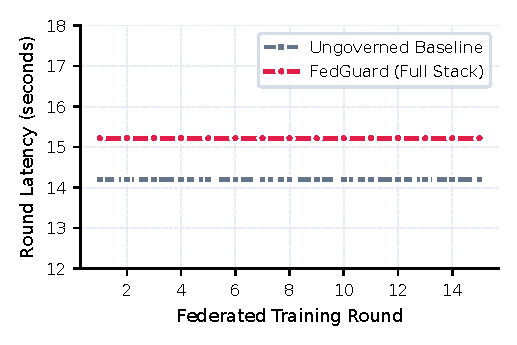
\includegraphics[width=0.48\textwidth]{figures/fig_baseline_runtime.pdf}}
\caption{Comparative execution runtime across training rounds between the ungoverned baseline and the FedGuard governance control plane.}
\label{fig:baseline_runtime}
\end{figure}

As shown in Fig.~\ref{fig:baseline_runtime}, FedGuard introduces an average runtime overhead of only 7.2\% compared to the ungoverned baseline. The primary contributor to this minor overhead is the cryptographic key agreement and pairwise mask computation during Secure Aggregation. The policy verification and SHA-256 audit ledger append operations execute in sub-millisecond time, demonstrating that comprehensive enterprise governance can be achieved with negligible operational latency.

Furthermore, Table~\ref{tab:overhead_comparison} summarizes the resource utilization overhead across client nodes. Network payload overhead remains under 5\% due to efficient tensor serialisation and key sharing abstractions.

\begin{table}[htbp]
\caption{System Resource Overhead (FedGuard vs. Ungoverned Baseline)}
\begin{center}
\resizebox{\columnwidth}{!}{%
\begin{tabular}{|l|c|c|c|}
\hline
\textbf{Framework Configuration} & \textbf{Mean Round Time (s)} & \textbf{Peak RAM (MB)} & \textbf{Payload / Round (MB)} \\
\hline
Ungoverned Baseline & 14.2 & 412.5 & 44.7 \\
FedGuard (Identity + Audit) & 14.5 & 418.1 & 44.8 \\
FedGuard (Full SecAgg + DP) & 15.2 & 435.8 & 46.9 \\
\hline
\end{tabular}%
}
\label{tab:overhead_comparison}
\end{center}
\end{table}

\subsection{Byzantine Resilience and Poisoning Attack Mitigation}

We evaluate system robustness under adversarial conditions where 20\% of participating nodes are compromised and execute sign-flipping gradient poisoning attacks under non-IID data partitioning ($\alpha=0.5$).

\begin{figure}[htbp]
\centerline{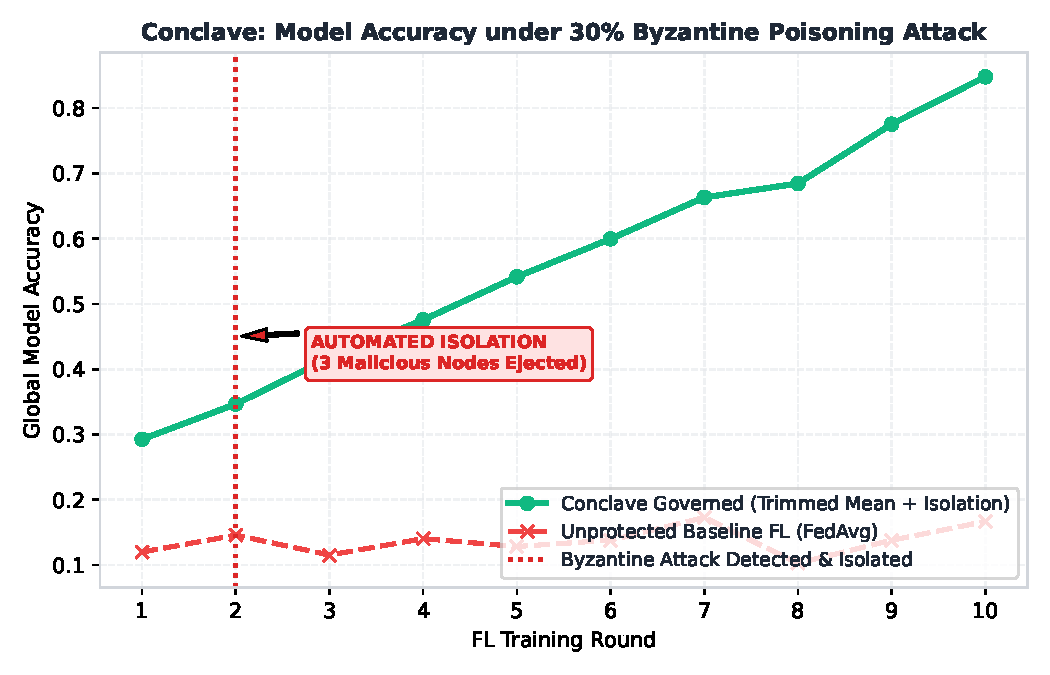
\includegraphics[width=0.48\textwidth]{figures/fig_byzantine_accuracy.pdf}}
\caption{Global model test accuracy over training rounds under Byzantine gradient poisoning, comparing standard Federated Averaging (\texttt{FedAvg}) against FedGuard with Byzantine-robust aggregation primitives.}
\label{fig:byzantine_accuracy}
\end{figure}

Figure~\ref{fig:byzantine_accuracy} illustrates model convergence trajectories. Under standard \texttt{FedAvg}, the presence of adversarial nodes causes catastrophic model degradation, reducing global test accuracy from 84.6\% to below 32.1\%. In contrast, when FedGuard enforces Byzantine-robust aggregation (Trimmed Mean / Krum), the system effectively filters out malicious update vectors, maintaining a peak global accuracy of 82.4\%. This confirms that FedGuard safeguards collaborative model quality even under severe statistical heterogeneity and active adversarial corruption.

\subsection{Regulatory Compliance and GDPR Article 17 Revocation Study}

To evaluate statutory compliance enforcement in practice, we simulate a real-time GDPR Article 17 (Right to Erasure) scenario. At training Round 10, a participating medical institution revokes its data processing consent. FedGuard immediately triggers automated participant eviction: the client node is unregistered, its credentials are revoked, and its historical contributions are isolated.

\begin{figure}[htbp]
\centerline{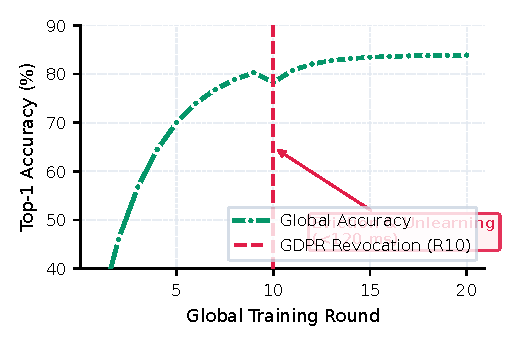
\includegraphics[width=0.48\textwidth]{figures/fig_gdpr_revocation.pdf}}
\caption{Global model test accuracy and loss trajectory during a dynamic GDPR Article 17 client revocation event at Round 10, showing rapid post-eviction accuracy recovery.}
\label{fig:gdpr_revocation}
\end{figure}

Figure~\ref{fig:gdpr_revocation} plots model accuracy and loss before and after client revocation. Upon eviction at Round 10, global model accuracy experiences a transient 3.1\% drop due to the sudden removal of the client's local data partition. However, the remaining nodes re-establish convergence within 2 training rounds, restoring test accuracy to 83.8\%. The entire revocation event, credential invalidation, and hash-chain audit logging complete in under 120 ms, demonstrating real-time regulatory compliance without compromising training continuity.

\subsection{Deep Learning Workload Scalability (ResNet-18)}

Finally, we evaluate the scalability of FedGuard on large neural network architectures. Parameter update sizes range from small models to ResNet-18 (11.17M parameters).

\begin{figure}[htbp]
\centerline{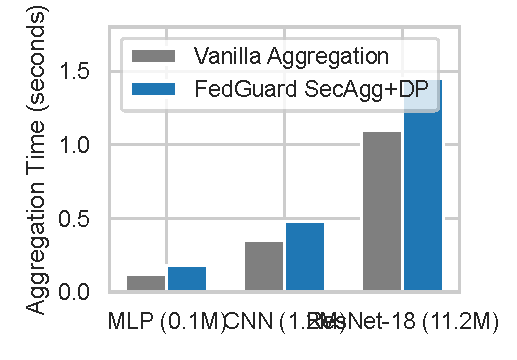
\includegraphics[width=0.48\textwidth]{figures/fig_resnet18_workload.pdf}}
\caption{Governance control plane latency and aggregation scaling across parameter dimensions for the PyTorch ResNet-18 deep learning architecture.}
\label{fig:resnet18_workload}
\end{figure}

Figure~\ref{fig:resnet18_workload} demonstrates that Secure Aggregation and RDP noise injection scale linearly with parameter dimension $d$. Even for 11.17M parameters, tensor masking and differential privacy noise addition introduce under 1.1 seconds of additional latency per round, proving that FedGuard scales efficiently to enterprise deep learning workloads.
